\chapter{Large-Scale Matrix Equations}

\section{Sparse Matrices}

Many matrices arising in applications are sparse.
For example, the shape regularity of the space triangulation of a \ac{PDE}
implies that each node has about the same number of neighbors,
and that number mainly depends on the space dimension of the problem.
For the matrix corresponding to that triangulation,
this number of neighbors determines the number of non-zero entries in the column or row corresponding a particular node.

\begin{example}[Sparsity of Steel Profile]
  The system matrices of the steel profile benchmark \cite{morwiki_steel} of size $n=371$ are sparse.
  Their spy plots are shown in \autoref{fig:spy} the number of non-zero entries $\nnz(\optional{})$ per matrix.
  $E$ has 4 to 11 entries per row, $A$ has 3 to 11, both having about \num{6.3} entries per row on average.
  For a uniform mesh of equilaterals covering~$\R^2$ that number would be \num{6}.
\end{example}

The common idea to represent a sparse matrix in memory is to only store the non-zero entries as well as their location within the matrix.
Perhaps the most common implementation is the so-called Compressed Column Storage (CCS),
sometimes called Compressed Sparse Column (CSC) format.
It's the format that \eg MATLAB\footnote{\url{https://www.mathworks.com/help/pdf_doc/otherdocs/simax.pdf}}
and Julia\footnote{\url{https://docs.julialang.org/en/v1.6/stdlib/SparseArrays/}} use by default.

\begin{figure}[t]
  \centering
  \begin{minipage}[c]{0.5\textwidth}
    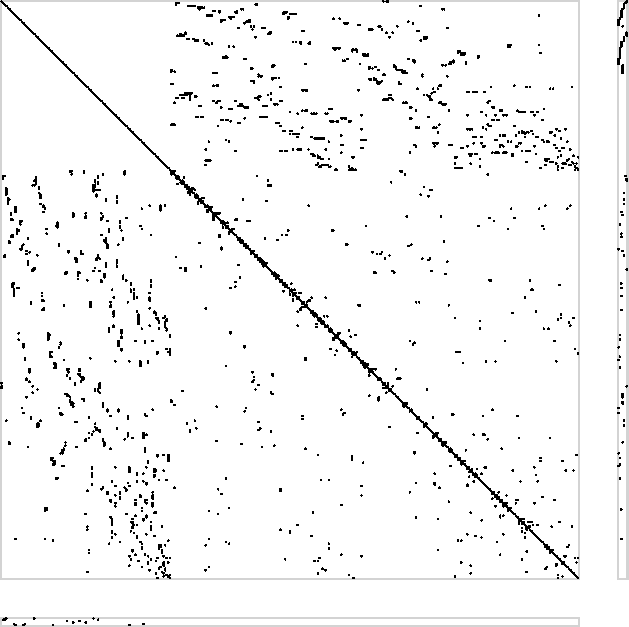
\includegraphics[width=\textwidth]{figures/spy_ABC.pdf}
  \end{minipage}
  \begin{minipage}[c]{0.25\textwidth}
    \flushright
    \begin{tabular}{cS[table-format=4.0]}
      \toprule
      & {$\nnz(\optional{})$} \\
      \midrule
      $E$ & 2343 \\
      $A$ & 2341 \\
      $B$ & 87 \\
      $C$ & 17 \\
      \bottomrule
    \end{tabular}
  \end{minipage}
  \caption[Sparsity pattern of Rail problem]{%
    Sparsity pattern of $A$, $B$ (right), and $C$ (bottom) of Rail problem for $n=371$,
    as well as their number of non-zero entries $\nnz(\optional{})$.
    The pattern of $E$ looks very similar to the one of $A$, only having 2 entries more.
  }
  \label{fig:spy}
\end{figure}

\section{Sherman-Morrison-Woodbury Formula?}

\section{Low-Rank Representations}
\label{sec:lowrank}

Even for sparse system matrices $E, A, B, C$
the solution $X$ of a \ac{DRE} is in general dense.
However, it usually is of low numerical rank,
\cf \eg~\cite[Section~2.1.4]{Lang2017}
and~\cite[Sections~2.3.3 and~2.3.4]{Kuerschner2016}
and the references therein.
The same holds for the solution $X(\optional{})$ of a \ac{DRE},
which is motivated by the following example.

\begin{example}[Low-Rank Solution of Steel Profile]
  The solution of the steel profile benchmark \cite{morwiki_steel} is given by the generalized \ac{DRE}~\eqref{eq:basics:DRE},
  \begin{equation*}
  \left\{
  \begin{aligned}
    E^\T \dot X E &= C^\T C + A^\T X E + E^\T X A - E^\T X BB^\T X E \\
    E^\T X(t_0) E &= \tfrac{1}{100} C^\T C
    .
  \end{aligned}
  \right.
  \end{equation*}
  Following \autoref{thm:basics:dre-limit-are},
  $X(\optional{})$ converges to $\bar X + \tilde C^\T \tilde C / 100$,
  $\tilde C = C E^{-1}$,
  where $\bar X$ is the (stabilizing) solution of the generalized \ac{ARE}
  \begin{equation*}
    0 = C^\T C + A^\T \bar X E + E^\T \bar X A - E^\T \bar X BB^\T \bar X E
  \end{equation*}
  \cf \eqref{eq:basics:ARE} having $S = BB^\T$ and $W = C^\T C$.
  That is, on one end of the time span $X$ has rank $q=6$
  while on the other end it converges to a matrix of numerical rank $113$.
  As the corresponding optimal control has some form of minimal energy,
  one can expect the numerical rank of the solution $X(\optional{})$ to depend on the ranks of initial and limit value,
  and to be not much larger in between.
  For this particular example that's about $\frac{1}{3}n$,
  which means the storage requirement of a single matrix can ideally be reduced by about $\frac{2}{3}$.
\end{example}

\paragraph{Classical Formulation}

As $X\in\Rnn$ is symmetric and positive semi-definite,
the classical approach would be a \ac{LRCF} $X=ZZ^\T$
for $Z \in\R^{n\times r}$, $r\ll n$.
The idea is then to only compute the low-rank factor $Z$
and never evaluate the full $X$.
This requires low-rank formulations for addition and subtraction of low-rank matrices.
Let $AA^\T$ and $BB^\T \in\Rnn$ be defined.
While an update for the \ac{LRCF} is straight-forward,
\begin{equation}
  AA^\T + BB^\T =
  \begin{bmatrix}
    A & B
  \end{bmatrix}
  \begin{bmatrix}
    A^\T \\ B^\T
  \end{bmatrix}
  ,
\end{equation}
a downdate is more involved.
One option is to use complex arithmetic, \ie
\begin{equation}
  AA^\T - BB^\T =
  \begin{bmatrix}
    A & \im B
  \end{bmatrix}
  \begin{bmatrix}
    A^\T \\ \im B^\T
  \end{bmatrix}
\end{equation}
where $\im^2=-1$.
This has several drawbacks, though.
The mathematical one is that we expect a real-valued solution to the \ac{DRE}.
Hence, the imaginary part should converge to zero quickly,
or there should be an equivalent real-valued factorization.
This leads to the technical drawback of a factor-2 overhead of complex arithmetic over real arithmetic.

Another option is therefore to handle the parts separately which are added versus subtracted in the superposition.
The actual difference is then only computed at the very end.
While this may only require updates,
the overall result suffers from numerical cancellation
\cite[50]{Lang2015}
\cite[\pno~186, thesis~10]{Lang2017}.

\paragraph{Indefinite Formulation}

A different strategy to represent matrices of low numerical rank is the \ac{LRSIF} \cite{Benner2009,Lang2015}
$X = LDL^\T$ for $L\in\R^{n\times r}$ and $D\in\R^{r \times r}$, $D=D^\T$, $r\ll n$.
This factorization does not require up- and downdate to be handled separately,
\begin{equation}
  ACA^\T \pm BDB^\T =
  \begin{bmatrix}
    A & B
  \end{bmatrix}
  \begin{bmatrix}
    C \\ & \pm D
  \end{bmatrix}
  \begin{bmatrix}
    A^\T \\ B^\T
  \end{bmatrix}
\end{equation}
for $A, B, C, D$ of compatible dimensions.
The inner dimension $r$ is in this thesis sometimes referred to as the rank of the factorization,
even though it's only an upper bound to which.

\begin{remark}
  Despite its name, $L$ does not need to be (lower) triangular.
  Similarly, $D$ does not need to be diagonal.
  In fact, the main results of \cite{Lang2015} are only due to non-diagonal $D$,
  and are repeated in \autoref{sec:ros}.
\end{remark}

If all matrices have full rank $\rank ABA^\T = r_1$ and $\rank CDC^\T = r_2$,
the resulting object $GSG^\T$ has inner dimension $r_1 + r_2$ but $\rank GSG^\T \leq r_1 + r_2$.
If the overall result is expected to have a low rank,
that inner dimension must not grow arbitrarily.
\autoref{alg:lowrank:compression} shows how to compress a \ac{LRSIF}
based on the most significant eigenvalues,
without imposing a maximum-rank condition,
\cf~\cite[Section~6.3.3]{Lang2017}.
The resulting factorization has a diagonal $D$ and (potentially) a lower inner dimension.

\begin{algorithm}[h]
  \caption{Column Compression for LRSIF}
  \label{alg:lowrank:compression}
  \KwIn{$G \in\Rnk$, $S\in\R^{k\times k}$, tolerance $0 < \epsilon \ll 1$}
  \KwOut{$G_r\in\Rnr$, $S_r\in\R^{r\times r}$ such that $G_r S_r G_r^\T \approx GSG^\T$ and $r \leq k$}
  Compute $G=QR\Pi^\T$ with $Q\in\Rnk$, $R\in\Rkk$ and a permutation $\Pi\in\Rkk$\;
  Compute a decomposition $R \Pi^\T S \Pi R^\T = V \Lambda V^\T$ with $V \in \Rkk$
  and a diagonal matrix $\Lambda\in\Rkk$ with diagonal entries $\abs{\lambda_1}\geq\ldots\geq\abs{\lambda_k}$\;
  % FIXME: this should be max{1, lambda_1}. Currently, it shouldn't do any harm as any X is psd,
  % and the RHS of the ALE should be as well. Check first stage of Ros2, though!
  % https://gitlab.mpi-magdeburg.mpg.de/jschulze/DifferentialRiccatiEquations.jl/-/issues/7
  Select $r \leq k$ such that $\abs{\lambda_r} \geq \epsilon\max\Set{1, \lambda_1} \geq \abs{\lambda_{r+1}}$\;
  $G_r \gets Q V_r$\;
  $S_r \gets \Lambda_r$\;
  \Comment{%
    $V_r$ consists of the first $r$ columns of $V$ and $\Lambda_r$ of the first diagonal block of $\Lambda$
  }
\end{algorithm}

\section{Model Order Reduction}

The goal of model order reduction is to find a so-called \ac{ROM}
\begin{equation}
\left\{
\begin{aligned}
  \hat E \dot{\hat x} &= \hat A \hat x + \hat B u \\
  \hat y &= \hat C \hat x
\end{aligned}
\right.
\end{equation}
to the \ac{FOM}~\eqref{eq:basics:system:generalized},
where the \ac{ROM} has fewer internal states $\hat x(t) \in\R^{\hat n}$
than the \ac{FOM} $x(t) \in\R^n$, $\hat n \ll n$.
The details are beyond the scope of this thesis,
refer to \eg~\cite{Antoulas2005,BennerMehrmannSorensen2005,Benner2021} for an introduction to the topic.
\todo{Does it, though? Is the solution of a DRE based on a ROM even low-rank? If the ROM has less than \eg 100 states, that's less than the rank of the ARE solution.}
In the end, computing the optimal control for the \ac{ROM} requires the same techniques as presented in this thesis.
